%%%%%%%%%%%%%%%%%%%%%%%%%%%%%%%%%%%%%%%%%%%%%%%%%%%%%%%%%%%%%%%%%%%%%%%%%%%%%%%%
%2345678901234567890123456789012345678901234567890123456789012345678901234567890
%        1         2         3         4         5         6         7         8

\documentclass[letterpaper, 10 pt, conference]{ieeeconf}  % Comment this line out
                                                          % if you need a4paper
%\documentclass[a4paper, 10pt, conference]{ieeeconf}      % Use this line for a4
                                                          % paper

%\IEEEoverridecommandlockouts                              % This command is only
                                                          % needed if you want to
                                                          % use the \thanks command
%\overrideIEEEmargins
% See the \addtolength command later in the file to balance the column lengths
% on the last page of the document

\usepackage[pdftex]{graphicx}
\graphicspath{{resources/}}

\usepackage{ifthen}

\usepackage{amssymb}

% The following packages can be found on http:\\www.ctan.org
%\usepackage{graphics} % for pdf, bitmapped graphics files
%\usepackage{epsfig} % for postscript graphics files
%\usepackage{mathptmx} % assumes new font selection scheme installed
%\usepackage{times} % assumes new font selection scheme installed
%\usepackage{amsmath} % assumes amsmath package installed
%\usepackage{amssymb}  % assumes amsmath package installed
\usepackage[T1]{fontenc}
\usepackage[utf8]{inputenc}
\usepackage{xspace}  
\usepackage{cite}  
\usepackage{ifthen}

% proof-reading
\usepackage{xcolor}
\usepackage[normalem]{ulem}
\newcommand{\ra}{$\rightarrow$}
\newcommand{\ugh}[1]{\textcolor{red}{\uwave{#1}}} % please rephrase
\newcommand{\ins}[1]{\textcolor{blue}{\uline{#1}}} % please insert
\newcommand{\del}[1]{\textcolor{red}{\sout{#1}}} % please delete
\newcommand{\chg}[2]{\textcolor{red}{\sout{#1}}{\ra}\textcolor{blue}{\uline{#2}}} % please change
\newcommand{\chk}[1]{\textcolor{ForestGreen}{#1}} % changed, please check

% comments \nb{label}{color}{text}
\newboolean{showcomments}
\setboolean{showcomments}{true}
\ifthenelse{\boolean{showcomments}}
	{\newcommand{\nb}[3]{
		{\colorbox{#2}{\bfseries\sffamily\scriptsize\textcolor{white}{#1}}}
		{\textcolor{#2}{\sf\small$\blacktriangleright$\textit{#3}$\blacktriangleleft$}}}
	 \newcommand{\version}{\emph{\scriptsize$-$Id$-$}}}
	{\newcommand{\nb}[3]{}
	 \newcommand{\version}{}}
\newcommand{\damien}[1]{\nb{Damien}{red}{#1}}
\newcommand{\serge}[1]{\nb{Serge}{blue}{#1}}
\newcommand{\pierrick}[1]{\nb{Pierrick}{green}{#1}}

% Hyphenate CamelCaseWords before each uppercase letter
\makeatletter
\newcommand{\camelhyph}[1]{\@fterfirst\c@amelhyph#1\relax }
\def\@fterfirst #1#2{#2#1}
\def\c@amelhyph #1{%
 \ifthenelse{\equal{#1}\relax}{}{%  Do nothing if the end has been reached
   \ifnum`#1<91 \-#1\else#1\fi%     Check whether #1 is an uppercase letter,
                              %     if so, print \-#1, otherwise #1
  \expandafter\c@amelhyph%    %     insert \c@amelhyph again.
}}
 
\makeatother

\newcommand{\diaspec}{Dia\-Spec\xspace}
\newcommand{\ct}[1]{\texttt{\camelhyph{#1}}}
\newcommand{\ie}{\emph{i.e.,}}
\newcommand{\eg}{\emph{e.g.,}}
\newcommand{\etc}{\emph{etc}}
\newcommand{\etal}{\emph{et al.}}

\title{Using the \diaspec{} design language and compiler to develop
  robotics systems}

\author{%
  \parbox{2.4 in}{\centering Damien Cassou\\
    Software Architecture Group, HPI\\
    University of Potsdam, Germany\\%
    {\tt\small damien.cassou@hpi.uni-potsdam.de}}
  \hspace*{ 0.1 in}
  \parbox{2.35 in}{ \centering Serge Stinckwich\\
UMMISCO, UMI 209\\IRD/IFI/Vietnam National University
    {\tt\small serge.stinckwich@ird.fr}}
  \hspace*{ 0.1 in}
  \parbox{1.9 in}{ \centering Pierrick Koch\\
CNRS, UMR 6072 GREYC\\ F-14032 Caen, France\\
    {\tt\small pierrick.koch@unicaen.fr}}
}

\usepackage{listings}

\lstdefinelanguage{diaspec}
{morekeywords={import, entity, attribute, extends, source, action, controller,
    context, from, on, void, Integer, Boolean, Float, String, enumeration,
    structure, indexed, by, as, include, when, get, no, maybe, always,
    publish, interaction, required, provided, abstract, do, any},%
  sensitive=true,
  morecomment=[l]{//},
  morecomment=[s]{/*}{*/},
}

\lstset{
    keywordstyle=\bfseries,
    basicstyle=\scriptsize\ttfamily,
    commentstyle=\ttfamily,
    stringstyle=\rmfamily,
    numbers=left,%none,%left,%
    numberstyle=\tiny,%\scriptsize,%\tiny
    stepnumber=1,
    numbersep=2pt,
    numberfirstline=true,       %
    numberblanklines=true,     %
    showstringspaces=false,
    breaklines=true,
    breakatwhitespace=true,
%    frameround=ftff,
%    frame=single,
    belowcaptionskip=.75\baselineskip,
    captionpos=b,
    numberbychapter=false,
    escapechar=\#
    %frame=L
} 
\usepackage[pdftex, colorlinks=true, urlcolor=black, linkcolor=black]{hyperref}
\begin{document}

\maketitle
\thispagestyle{empty}
\pagestyle{empty}


%%%%%%%%%%%%%%%%%%%%%%%%%%%%%%%%%%%%%%%%%%%%%%%%%%%%%%%%%%%%%%%%%%%%%%%%%%%%%%%%
\begin{abstract}

  A Sense/Compute/Control (SCC) application is one that interacts with
  the physical environment. Such applications are pervasive in domains
  such as building automation, assisted living, and autonomic
  computing. Developing an SCC application is complex because: (1) the
  implementation must address both the interaction with the
  environment and the application logic; (2) any evolution in the
  environment must be reflected in the implementation of the
  application; (3) correctness is essential, as effects on the
  physical environment can have irreversible consequences.

  The SCC architectural pattern and the \diaspec{} domain-specific
  design language propose a framework to guide the design of such
  applications. From a design description in \diaspec{}, the
  \diaspec{} compiler is capable of generating a programming framework
  that guides the developer in implementing the design and that
  provides runtime support. In this paper, we report on an experiment
  using \diaspec{} (both the design language and compiler) to develop
  a standard robotics application. We discuss the benefits and
  problems of using \diaspec{} in a robotics setting and present some
  changes that would make \diaspec{} a better framework in this
  setting.

\end{abstract}

%!TEX root=dslrob.tex
\section{Introduction}

A Sense/Compute/Control (SCC) application is one that interacts with
the environment~\cite{Tayl09a}. The SCC architectural pattern
guides the description of SCC applications and involves four kinds of
components, organized into layers~\cite{Cass11a,Edwar09a}: (1)
\emph{sensors} at the bottom, which obtain information about the
environment; (2) then \emph{context operators}, which process this
information; (3) then \emph{control operators}, which use this refined
information to control (4) \emph{actuators} at the top, which finally
impact the environment. A robotics application is a kind of SCC
application where the environment is composed of a robot
(sensors/actuators/body, control architecture, \etc{}) and the robot's
neighborhood (the walls, ground, people, \etc{})~\cite{Sicil08a}. As
noticed by Taylor \etal{}~\cite{Tayl09a}, the Sense/Plan/Act
architecture~\cite{Sicil08a}, widely used in robotics, closely
resembles the SCC architectural pattern.

\diaspec{} is a domain-specific design language dedicated to
describing SCC applications~\cite{Cass09b,Cass11a}. From such a design
description, the \diaspec{} compiler produces a dedicated Java
programming framework that is both \emph{prescriptive} and
\emph{restrictive}: it is prescriptive in the sense that it guides the
developer, and it is restrictive in the sense that it limits the
developer to what the design description allows. By separating
application logic (implemented by the developers) and runtime support
(generated in the programming framework), \diaspec{} facilitates the
design, implementation and evolution of SCC applications.

%\damien{Talk about problems in the robotics domain: ad-hoc solutions, hard to reuse, hard to adapt to new environments...}

\subsection*{Contributions}

Our contributions are as follows:

\begin{itemize}
\item \emph{A report} on an experiment of designing and implementing a
  standard robotics application in the SCC architectural pattern with
  the \diaspec{} domain-specific design language and framework
  (Sections~\ref{sec:designing} and~\ref{sec:implementing}). This
  report includes detailed instructions and guidelines to allow
  further experiments.
\item \emph{A discussion} of the benefits and problems of using
  \diaspec{} in a robotics setting (Section~\ref{sec:discussing}).
  This discussion includes a list of changes to \diaspec{} that would
  make it a better framework for developing new robotics applications.
\end{itemize}

We finally highlight some related works and conclude in
sections~\ref{sec:related} and~\ref{sec:conclusion}.

%%% LocalWords:  SCC




%!TEX root=dslrob.tex
\section{Designing a robotics application}
\label{sec:designing}

In this section we first explain how to decompose a robotics
application in \diaspec{} component types. Then we present a case
study that we use as an example of how to describe a robotics
application with \diaspec{}.

In the rest of this paper we are going to take
ROS\footnote{\url{http://www.ros.org/wiki/}} as the underlying
middleware for our case study. We believe it is a good choice as ROS
is becoming a standard within the robotics community. It is important
to note however that our approach and \diaspec{} are completely
independent of any middleware.

\subsection{Decomposing}

Designing an application with \diaspec{} requires a decomposition in
layers. Each layer corresponds to a separate type of component:

\begin{itemize}
\item A \emph{sensor} sends information sensed from the environment to
  the context operator layer through data \emph{sources}. A sensor can
  both push data to context operators and respond to context operator
  requests. We use the term ``sensor'' both for entities that actively
  retrieve information from the environment, such as system probes,
  and entities that store information previously collected from the
  environment, such as structured information coming from the
  middleware.
\item A \emph{context operator} refines (aggregates and interprets)
  the information given by the sensors. Context operators can push
  data to other context operators and to control operators. Context
  operators can also respond to requests from parent context
  operators.
\item A \emph{control operator} transforms the information given by
  the context operators into orders for the actuators.
\item An \emph{actuator} triggers actions on the environment.
\end{itemize}

The following details the steps to follow in order to decompose a
robotics application into these component types.

\paragraph*{Reusing existing components}
In the presence of a previous application developed with \diaspec{},
it is possible and advisable to reuse as much components as possible.
Depending on the amount of reused components, this can have a huge
impact on the application of the other steps.
% shouldn't talk about middleware reuse here as it is discussed below:
% It is similarly important to reuse as much building blocks as
% possible from the underlying middleware. For example ROS provides
% high-level components and algorithms that are better reused than
% reimplemented.

\paragraph*{Listing capabilities}
Each robot comes with its own set of capabilities (\eg{} sensing
motion and projecting light). These capabilities should be mapped to
sensor sources and actuator actions. Related sources and actions
should then be grouped inside \emph{entity classes} (\eg{} a camera
providing a picture source and zooming action). Beside sources and
actions, an entity class may also have \emph{attributes} to
characterize its instances (\eg{} resolution, accuracy and status). In
the presence of a high-level middleware (such as ROS), it can be
useful to also map capabilities of the middleware into sources and
actions (\eg{} a mapping or a localization capability).

\paragraph*{Identifying main context operators}
The next step of the decomposition in components is the identification
of the main high-level pieces of information required by the
application. These pieces of information are represented as context
operators and directly used as input to control operators

\paragraph*{Decomposing into lower-level pieces}
Then, lower-level context operators must be identified to act as input
sources for the higher-level ones. This decomposition is typically
done in several steps, each step slightly lowering the level of
previously identified context operators. This decomposition ends when
each identified context operator can directly take its input from a
set of sensor sources. 

\paragraph*{Identifying control operators}
From the high-level context operators, it is then necessary to derive
a set of control operators that are going to send orders to actuators.
Because the code of a control operator can not be reused in another
part of the application, it is important that this code is as simple
as possible. If there is opportunity for reuse, the code should be
moved to a new context operator. 

\paragraph*{Identifying data types}
While proceeding with the above steps, it is also necessary to define
various data types. These types are used to describe entity sources,
context operators, and parameters of actuator actions. A data type is
either primitive (\eg{} integer, boolean and float), an enumeration of
names (\eg{} a luminosity can either be low, normal or high), or a
structure (\eg{} a coordinate with x and y fields). An important
question arises in the presence of a high-level middleware (such as
ROS): should the types of the application be the types provided by the
middleware or should the application define new types. The former
solution is easier to use whereas the latter provides more decoupling.
A general principle is to provide new types when their transcription
in \diaspec{} is straightforward (\eg{} a coordinate) and to reuse the
middleware types otherwise (\eg{} ROS defines a ``twist'' data type
that is complex enough to not be reimplemented).

\subsection{Case Study}

\serge{Il faut préciser quelque part le modèle de robot et le type de locomotion.}

As a running example, we present an application that is typical of the
robotics domain. In this application, a robot evolves in an unknown
environment and has two modes: \emph{random} and \emph{exploration}.
In the random mode, the robot goes straight and when an obstacle is
close enough turns before going straight again. In the exploration
mode, the robot goes to unvisited locations with the goal to visit as
much as possible from the neighborhood. The current mode can be
changed anytime by an operator through a graphical interface. In both
modes, the robot turns on an embedded projector and takes pictures
when it is in a zone with obstacles.

\serge{Il faut préciser l'algorithme d'exploration}

Let us now discuss the above steps in the context of this case
study (Figure~\ref{fig:diaspec-graph} represents the result).

\begin{figure}
  \centering
  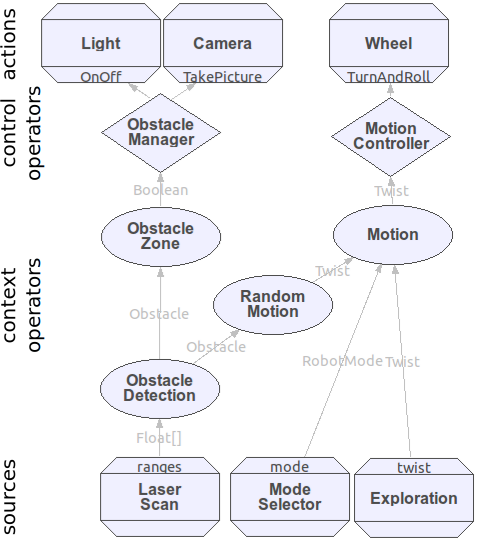
\includegraphics[width=.7\linewidth]{diaspec-graph}
  \caption{The case study decomposed into the different type of
    components of \diaspec{}}
\label{fig:diaspec-graph}
\end{figure}

\paragraph*{Reusing existing components}
We assume no previous \diaspec{} application and thus no \diaspec{}
component to reuse.

\paragraph*{Listing capabilities}
Our robot comes with a range-finder type laser scanner, a light projector, a camera,
and a set of wheels. We are reusing \emph{exploration} capability developed by Bosch robotics research team\footnote{\url{http://www.ros.org/wiki/explore}} and available as a ROS node. That is exactly what we need for the
robot's exploration mode. From all these capabilities, we identify:
\begin{itemize}
\item a \ct{LaserScan} entity class with a \ct{ranges} source
  providing laser ranges from the sensor which can be deactivated when
  the robot is in exploration mode;\footnote{it is important to note
    that the application is not going to deactivate the hardware-level
    sensor (which is used in the two modes) but only the
    application-level source (which is only used in the random mode).}
\item A \ct{ModeSelector} entity that provides a graphical interface
  for the operator to choose the robot's current mode.
\item an \ct{Exploration} entity that provides a source of twists for
  the robot;
\item a \ct{Light} and \ct{Camera} entities that respectively take
  pictures and enlighten the neighborhood on request;
\item a \ct{Wheel} entity that can turn or roll on request;
\end{itemize}

\paragraph*{Identifying main context operators}
The most important activity of our robot is to move. Therefore we
introduce a \ct{Motion} context operator that produces a twist,
representing the robot's motion. Because our robot takes pictures and
turns on its projector when it is in a zone with obstacles, we
introduce an \ct{ObstacleZone} context operator that indicates whether
or not some obstacles are in the neighborhood.

\paragraph*{Decomposing into lower-level pieces}
The \ct{Motion} context operator produces a twist based on which mode
is currently selected and on the twist values coming from both modes.
The currently selected mode is directly provided by the
\ct{ModeSelector} entity. We introduce a \ct{RandomMotion} context
operator that produces random twists. The twist for the exploration
mode is directly provided by the \ct{Exploration} entity. Both the
\ct{ObstacleZone} and \ct{RandomMotion} context operators need the
information about nearby obstacles. We thus introduce the
\ct{ObstacleDetection} context operator to indicate the proximity of
an obstacle.

\paragraph*{Identifying control operators}
The \ct{MotionController} control operator takes information from the
\ct{Motion} context operator and transmit this information to the
\ct{Wheel} entity. The \ct{ObstacleManager} control operator takes
information from the \ct{ObstacleZone} context operator and triggers the
light and takes a picture with the camera.

\paragraph*{Idenfiying data types}
We have already seen that our application uses the notion of twist to
indicate motion. A twist can be defined as a pair of vector which
represent the linear and angular velocity. The robot current mode is
represented as an enumeration of the \ct{RANDOM} and \ct{EXPLORATION}
names. The \ct{ObstacleDetection} context operator provides an
\ct{Obstacle} data type containing both a boolean to indicate if an
obstacle is in front of the robot and a set of float numbers (the
ranges) as provided by the laser scan giving details about the
neighborhood.

\subsection{Describing with \diaspec{}}

Once the application is decomposed using the different component
types, the transcription to the \diaspec{} design language is
straightforward. Listing~\ref{listing:design} gives an extract of the
case study transcription.\footnote{The full case study description in
  \diaspec{} and implementation can be found in
  \url{http://github.com/DamienCassou/diarobot}.}

\lstinputlisting[float,language=diaspec,breakatwhitespace=true%
,caption={An extract of the description of the robotics application
  with the \diaspec{} design language}%
,label={listing:design}]%
{code/design.diaspec}

In this listing, the \ct{entity}, \ct{context}, and \ct{controller}
keywords are respectively used to introduce a new entity class, a new
context operator, and a new control operator. For this application, we
decide to reuse the \ct{Twist} data type of the ROS middleware which
is illustrated in line~\ref{design:import}.

Additionally to the description of an operator's input sources, the
\diaspec{} language allows each operator to describe a set of
\emph{interaction contracts} that coordinate these input sources. An
interaction contract is a tuple that describes an \emph{activation
  condition} indicating which input sources can activate the operator
and a \emph{reaction} indicating what to do as a result of the
activation condition.\footnote{Previous work~\cite{Cass11a} also
  includes in the tuple a set of \emph{data requirements} indicating
  the additional input sources that can be used for a particular
  activation condition. This is not used in this case study.} The
\ct{interaction} keyword is used to introduce an interaction contract.
For example, the \ct{ObstacleDetection}'s interaction contract
(Listing~\ref{listing:design}, line~\ref{design:interaction})
indicates that this context operator always publishes a data when it
receives information from the laser scan.

In this section we saw how to design a robotics application using
the SCC architectural pattern and the \diaspec{} design language. Both
the pattern and the language help decomposing an application in well
defined components. Both make it easy to reuse as much as possible
from the underlying middleware and existing applications. In the next
section we discuss how to implement a robotics application with our
approach.

%%% Local Variables:
%%% mode: latex
%%% coding: utf-8
%%% TeX-master: "dslrob"
%%% TeX-PDF-mode: t
%%% ispell-local-dictionary: "english"
%%% End:

% LocalWords:  boolean

%!TEX root=dslrob.tex

\section{Implementing a robotics application}
\label{sec:implementing}

The \diaspec{} compiler generates a programming framework with respect
to a set of declarations for entity classes, context operators and
control operators (Figure~\ref{fig:diaspec-process}). For each
component description (entity or operator) the compiler generates an
abstract class. The abstract methods in this class represent code to
be provided by the developer (\emph{hole} in
Figure~\ref{fig:diaspec-process}), to allow him to program the
application logic (\eg{} to trigger an entity action) (\textit{bump}
in Figure~\ref{fig:diaspec-process}).

\begin{figure}[ht]
  \centering
  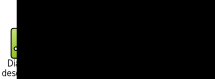
\includegraphics[width=\linewidth]{diaspec-process}
  \caption{Overview of the \diaspec{} development process}
  \label{fig:diaspec-process}
\end{figure}

Implementing a \diaspec{} component is done by \textit{sub-classing}
the corresponding generated abstract class. In doing so, the developer
is required to implement each abstract method. The developer writes
the application code in subclasses, not in the generated abstract
classes. This strategy contrasts with generating incomplete source
code, to be filled by the developer. As a result, in our approach, one
can change the \diaspec{} description and generate a new programming
framework without overriding the developer's code. The mismatches
between the existing code and the new programming framework are
revealed by the Java compiler. To facilitate the implementation
process, most Java IDEs are capable of generating class templates
based on super abstract classes.

In this section, we give an overview of how to implement some parts of
the case study. For a more detailed description, we refer to our
previous works~\cite{Cass09b,Cass11a,Cass11b}.

\subsection{Implementing an operator}

For each context or control operator, a dedicated abstract class is
generated in the programming framework. For each interaction contract
of this operator, the generated abstract class contains an
\emph{abstract method} and a corresponding \emph{calling method}. The
abstract method is to be implemented by the developer while the
calling method is used by the framework to call the implementation of
the abstract method with the expected arguments.

The signature of each abstract method is directly derived from the
interaction contract: the name of the method is derived from the
activation condition, the return type is derived from the reaction,
and the parameters are derived from the activation condition and the
reaction.

Listing~\ref{listing:contextop-implem} presents a possible Java
implementation of the \ct{RandomMotion} context operator. The
\ct{onObstacleDetection} method is declared abstract in the
\ct{AbstractRandomMotion} generated super class.

\lstinputlisting%
[float,language=java,%
caption={A developer-supplied Java implementation of the
  \texttt{Random\-Motion} context operator described in
  Listing~\ref{listing:design}. The \texttt{Abstract\-Random\-Motion}
  super class is automatically generated},%
label={listing:contextop-implem}]%
{code/RandomMotion.java}

Because an operator only manipulates input sources to produce a
result, its implementation is independent of any robotics software
framework. This facilitates operator reuse for different applications
and robots.

\subsection{Implementing an entity}

Contrary to operators which are dedicated to the application logic, an
entity is at the border between the application and its environment
(\eg{} the middleware and robot hardware). Implementing an entity thus
requires some knowledge of the underlying hardware or middleware.

Listing~\ref{listing:laserscan-implem} presents a possible Java
implementation of the \ct{LaserScan} entity class for the ROS
middleware. When the middleware publishes a new laser scan message,
this message is automatically received by the \ct{RosLaserScan}
instance through the ROS \ct{MessageListener} interface.

\lstinputlisting%
[float,language=java,%
caption={A developer-supplied Java implementation of the
  \texttt{LaserScan} entity class described in
  Listing~\ref{listing:design}, line~\ref{design:laserscan-b}. The
  \texttt{Abstract\-Laser\-Scan} super class is automatically
  generated},%
label={listing:laserscan-implem}]%
{code/RosLaserScan.java}

Listing~\ref{listing:light-implem} presents a possible Java
implementation of the \ct{Light} entity class for the ROS middleware.
The constructor receives a ROS \ct{publisher} as a parameter which
allows the entity implementation to send commands to the robot through
the middleware.

\lstinputlisting%
[float,language=java,%
caption={A developer-supplied Java implementation of the
  \texttt{Light} entity class described in
  Listing~\ref{listing:design}, line~\ref{design:light-b}. The
  \texttt{Abstract\-Light} super class is automatically generated},%
label={listing:light-implem}]%
{code/RosLight.java}

\subsection{Deploying an application}

Deploying an application requires writing a deployment script in Java.
To do this, a developer creates a new Java class by sub-classing the
abstract class \ct{MainDeploy} generated in the programming framework.
By doing so the developer is required to implement one abstract method
per operator, to call the \ct{add()} method to register entity
instances, and to call the \ct{deployAll()} method to trigger the
deployment. The ROS middleware requires an implementation of the
\ct{NodeMain} interface. An extract of the deployment script for the
case study application is shown in Listing~\ref{listing:deploy}.

\lstinputlisting%
[float,language=java,%
caption={An extract of a developer-supplied Java deployment script for
  the case-study application},%
label={listing:deploy}]%
{code/Deploy.java}


\begin{figure}
  \centering
 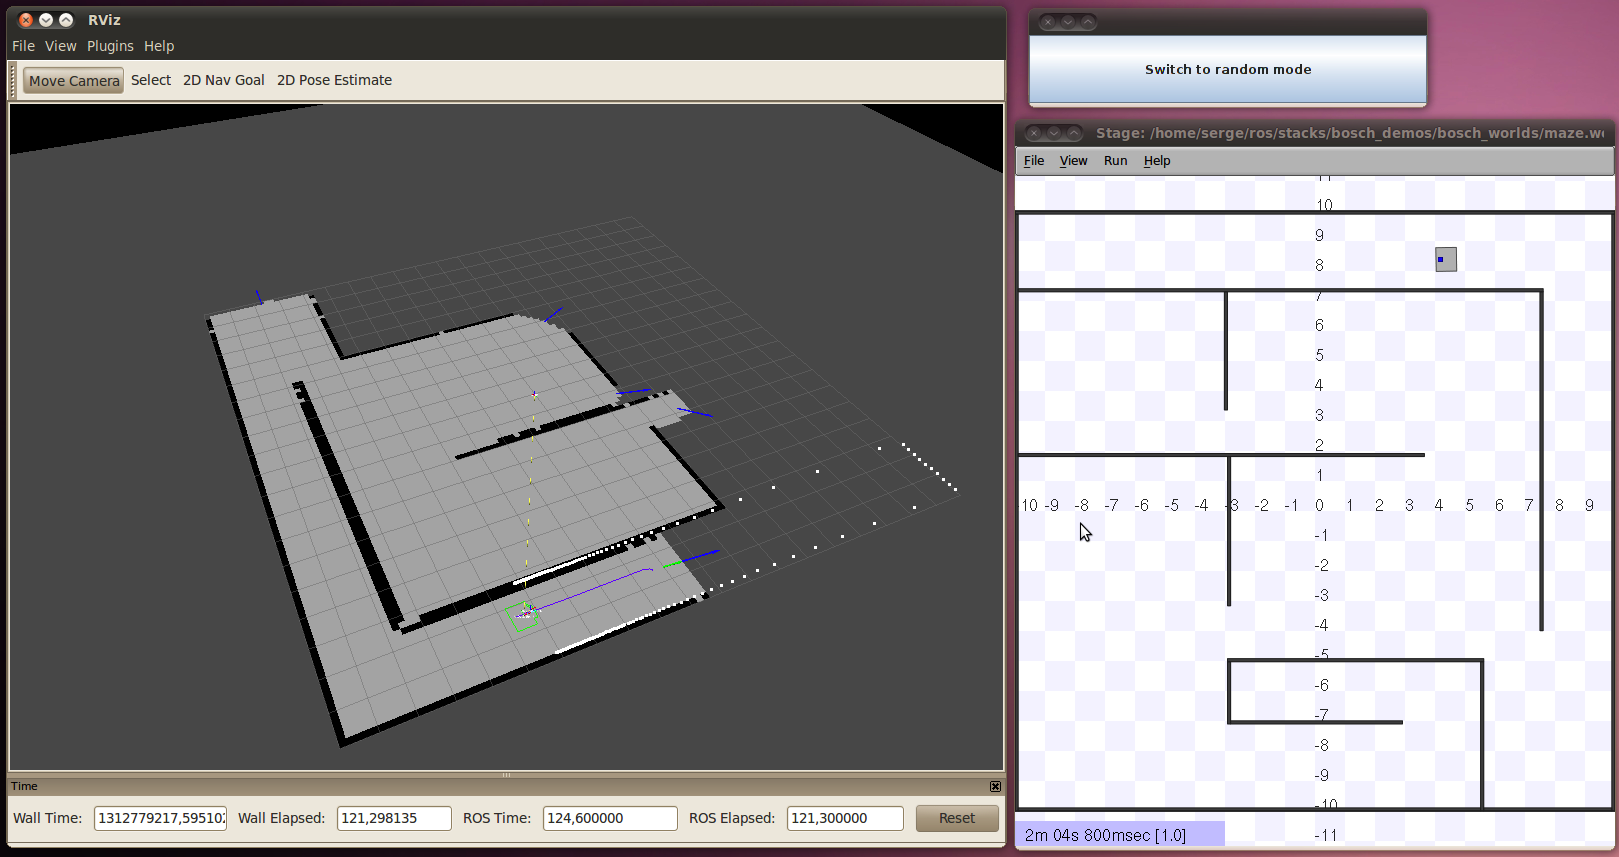
\includegraphics[width=1\linewidth]{capture}
  \caption{Screenshot of a simulation of the case study}
\label{fig:diaspec-simulation}
\end{figure}

In this section we saw how to implement a robotics application on top
of a programing framework generated by the \diaspec{} compiler. This
programming framework calls developer's code when necessary and make
the development easy by passing everything the developer needs as a
parameter to abstract methods. In the next section we discuss the
benefits and problems of using \diaspec{} in a robotics setting.

Figure~\ref{fig:diaspec-simulation}  presents a running simulation of our case study, where you can see ROS sensors visualization tool rivz on the left, a Stage simulation engine instance on the right and the button to switch between exploration and random mode on the top. The code generated is completely integrated in the ROS middleware and the execution can be analyzed by the tools provided by ROS.
\section{Discussing}
\label{sec:discussing}

A robotics application is mostly static and often contains only one
instance of each entity. This makes entity selection and subscription
mostly useless and they would better be done within the programming
framework.

Types can be reused from existing software frameworks, such as ROS.
This makes the whole application description and implementation
simpler. However, this also tightly couples the whole application to a
particular software framework, limiting reuse in other contexts.

%!TEX root=dslrob.tex

\section{Related Work}
\label{sec:related}

Several software engineering approaches have been proposed to lower
the complexity of robotics systems~\cite{Brug07a}.

Numerous middlewares and software frameworks have been proposed to
support the implementation of robotics applications (\eg{}
CLARATy~\cite{Claraty}, ROS~\cite{ROS} and Player~\cite{Coll05a}).
Such approaches attempt to cover as much of the robotics domain as
possible in a single programming framework. This strategy often leads
to large APIs, providing little guidance to the developer and
requiring boilerplate code to customize the programming framework to
the characteristics of the application. In contrast, a
\diaspec{}-generated programming framework specifically targets one
application, limiting the API to methods of interest to the
developers. Our code generator could potentially target these
middlewares thus leveraging existing work and completely hiding their
intricacies from the developer.

Component-based software engineering for robotics~\cite{Brug07b} and
model-driven software engineering for Robotics (e.g., OMG
RTC~\cite{OMGRTC}, SmartSoft~\cite{Schl09a}). All these approaches
apply and tailor general-purpose and established principles of
lowering complexity to robotics needs and come up with domain-specific
extensions.

Domain-specific languages for robotics (e.g Smach~\footnote{\url{http://www.ros.org/wiki/smach} Reference to add: J. Boren and S. Cousins, “The SMACH High-Level Executive [ROS News],” IEEE RAM, vol. 17, no. 4, pp. 18–20, 2010. }, SmartTCL~\footnote{Reference to add: Andreas Steck and Christian Schlegel, "Managing Execution Variants in Task Coordination by Exploiting Design-Time Models at Run-Time", in Proc. IEEE/RSJ Int. Conf. on Intelligent Robots and Systems (IROS), San Francisco, California, USA, September 2011. (to appear)}, ...).

Smach is a Python embedded DSL based on hierarchical concurrent state machines for composing complex robot behaviors from primitive ones.

SmartTCL (Smart Task Coordination Language) is an extension of CommonLisp that is used to do online dynamic reconfiguration of the software components involved in a robot: knowledge bases, simulation engines, symbolic task planners, models and low-level hardware. At design time, the developer defines execution variants that robot operates at runtime. In order to lower robotics inherent complexity, analysis and simulation tools could also be used at runtime to determine pending execution steps with specific parametrisation before the robot effectively execute them.

Dire qu'on a une approche dédiée.

Add to reference: David Kortenkamp, Reid Simmons, Chapter 8 - Robotic Systems Architectures and Programming, Handbook of Robotics, Springer Verlag.

%!TEX root=dslrob.tex

\section{Conclusions and future works}
\label{sec:conclusion}

In this paper, we have proposed to use \diaspec{}, a domain-specific
design language for Sense/Compute/Control applications, in a robotics
setting. We have shown how this language allows a developer to
structure an application in fine-grained and reusable components by
following the SCC architectural pattern. Developing a complex
application shows the benefits of such an approach in terms of reusing
existing software and lowering complexity for the developer. We have
also highlighted various problems we have met during the development
of a standard robotics application.

Being able to adapt a robotics system to different capabilities and
resources is a key issue in software engineering for robotics. For
example, two similar missions can be performed differently with
different resources on the robot. Our approach facilitates changes to
a robotics system by making explicit the software components and their
interactions. However supporting static adaptation is not enough in a
robotics setting as robots need to dynamically adapt to resource
evolutions (\eg{} failures and environment) while performing their
tasks. \emph{Resource-adaptive architectures} address dynamic
adaptations. However, such architectures are ad hoc solutions that can
not be reused and scaled. Therefore, an ideal robot control
architecture should be \emph{resource-adapting}, \ie{} an architecture
that explicitly manages and represents resources~\cite{Bour07a}. The
main perspective of this work is to introduce such dynamic variability
inside \diaspec{}.


\section{ACKNOWLEDGMENTS}

The authors gratefully acknowledge the INRIA Phoenix research group
who granted the authors the authorization of use of DiaSuite, a tool
suite which includes \diaspec{}.

\bibliographystyle{plainurl}
\bibliography{dslrob}

\end{document}

%%% Local Variables: 
%%% mode: latex
%%% TeX-master: t
%%% End:
